\documentclass{article}
\usepackage[utf8]{inputenc}
\usepackage[english]{babel}
\usepackage{hyperref}
\usepackage{amsmath}
\usepackage{amsfonts}
\usepackage{amssymb}
\usepackage{tikz}
\usetikzlibrary{calc}
\usepackage[square,numbers,sort&compress]{natbib}
\title{Bernstein Polynomials and the Weierstrass Theorem}
\author{Jishnu Kaiwar
  \and
  Bing En Gan
  \and
  Constantinos Azas}
\date{March 2019}
\begin{document}

\maketitle

\begin{abstract}
    In this paper, we will be studying Bernstein Polynomials and the Weierstrass Theorem.
    Bernstein Polynomial is a polynomial in Bernstein form, which has a number of useful applications.
    Bernstein Polynomials led to the discovery of Bezier curve which is widely used in computer graphics.
    Weierstrass Theorem states that any continuous function on $[0,1]$ can be uniformly approximated by polynomials.
    In this setting, we will present two proofs to the Weierstrass Theorem, one using the Bernstein polynomials to proof from definition, and the other using Bernstein's proof which is based on probability theory.
    The latter may not be the most straightforward proof, but it is easily the simplest and most elegant.
\end{abstract}
\newpage
\tableofcontents 
\newpage
\section{Introduction}\label{sec:intro}
Polynomials are one of the most fundamental expressions in Mathematics, consisting of variables and coefficients, which is widely used in all areas of Mathematics. Polynomials can be categorized into many different types, but we will be mainly discussing about Bernstein Polynomials here. First, we will begin with a brief history about the approximation theory. Then, we will move on to give an introduction about the Bernstein Polynomial, which is actually not something new if you did binomial distribution in Statistics. Then, we will move on to talk about the Weierstrass approximation theorem, which we will use the Bernstein Polynomial to proof the theorem. We will also include an alternative proof using the probability theorem, initially proved by Sergei Bernstein, which is thought to be the simplest and most elegant proof of the Weierstrass approximation theorem. Lastly, we will talk about application of Bernstein Polynomial, namely the Bezier Curve, which is broadly used in computer graphics.

\section{Brief History of the Problem}\label{sec:hist}
Karl Wilhelm Theodor Weierstrass (1815-1897) was a German mathematician whose contribution includes Abelian function, the theory of analytic function, elliptic functions, etc.
The Weierstrass approximation theorem was established by him in the 1885. 
The theorem says that polynomials can uniformly approximate any function that is continuous over a fixed interval.
The Taylor series expansion also gives the approximation of a given continuous function, however, it is only accurate near a given point $x_0$, but the approximation is usually not that good away from $x$.
Now, we will introduce the other mathematician that contributed to this problem, Sergei Bernstein (1880-1968), a Russian mathematician, whose main contributions to mathematics are in probability theory, approximation theory, etc. 
It was in 1908 that a Belgium mathematician, Charles Jean de La Vallee Poussin posed a question- is it possible to approximate the ordinate of a polygonal line by means of a polynomial of degree $n$ with error less than $1/n$.
It was the need to formulate a ``well-behaved'' polynomial that gave rise to the introduction of the Bernstein basis, and thus we will introduce the Bernstein polynomial, which is the linear combination of the Bernstein basis.
Both Charles Jean and Bernstein made some progress in the following years.
Finally, in 1911, Bernstein gave a complete solution, introducing what we call now as Bernstein polynomials and giving a proof of Weierstrass approximation theorem.
He submitted this thesis as \textit{About the Best Approximation of Continuous Functions by Polynomials of Given Degree} to receive his second doctorate from Kharkov University.
This thesis has also earned him a prize from the Belgium Academy of Science in 1911.\cite{o'connor_robertson_2010}
Now, moving on to Bezier Curves, they were first introduced into theoretical mathematics long before computers, primarily by French mathematician Charles Hermite and Russian mathematician Sergei Bernstein.
It was not until an employee of the automobile maker Renault, and of Paul de Casteljau, of Citroen, that brought these curves into computer graphics.\cite{farouki2012bernstein}
\section{Taylor Series vs Bernstein Polynomial}\label{sec:tsvsbp}
Our aim is to approximate continuous functions on a closed interval of the real axis. Approximation of functions is mainly based on finding tangent lines on specific points in the given interval. So on some linear polynomial we can approximate it by finding a tangent at a given point. But if you consider functions, for example, $\sin x$ or  $e^{x^2} $, they are much more difficult to approximate them using tangent lines of the form $f(x) =mx+b$, rather than linear functions. So in this case we use polynomials and so we use Taylor approximations on these polynomials. Basically, we use differentiable calculus to find tangent lines on some given values of $x$. Back in our case the idea of tangent lines can be extended using polynomials of higher degree which are somehow considered ``tangent'' on a given curve, of course for some values of $x$.
Let $p$ be a continuous function in the interval $[a,b]$. We can compute Taylor’s first degree polynomial $F_1(x)$ as $F_1(x)=p(r) + p'(r) (x – r)$, where $r\in[a,b]$ for $x$ `close' to $r$. If we want to consider Taylor’s second degree polynomial, we then can compute $F_2(x)= p(r) + p '(r) (x – r)+ \frac{1}{2!}p''(r) (x – r)^2$, where $r \in [a,b]$ for $x$ 'close' to r.
The graph of this approximating polynomial for $p$ is the tangent line.
\begin{equation*}
    y=p(r)+p'(r)(x-r) \ \text{at}\ x=r
\end{equation*}
\begin{figure}[h!]
\centering
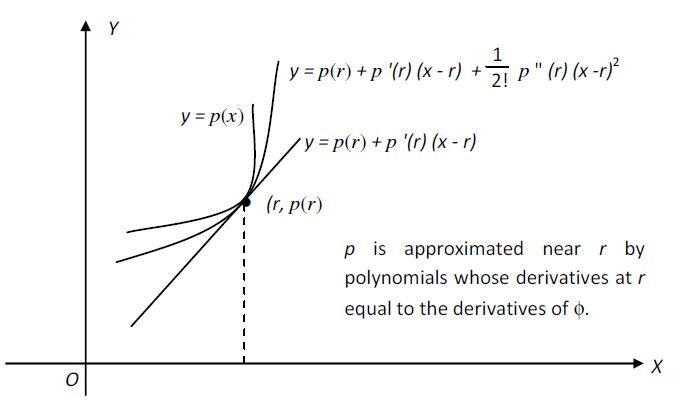
\includegraphics[width=1\textwidth]{Project-weierstrass.JPG}
    \caption{Graph of approximating polynomial for $p$}
    \label{fig:1}
\end{figure}

So we can from figure 1 that the polynomial $p$ could be a weird curve that it Is difficult to approximate it using a straight line of the form $y=mx+b$. So we use polynomials using the Taylor series.
But in general, the function $p$ on the closed interval $[a,b]$ can be approximated with Taylor series of the form $F_n(x) = p(r) + p'(r)(x – r) + \frac{1}{2!}p''(r) (x – r)^2 + … + \frac{1}{n!} p^n(r)(x – r)^n$ for $x$ `close' to $r$.
\paragraph{}
We have already shown that Taylor series, give a way of approximating continuous functions using polynomials on a closed interval. But this method does not specify approximations on the whole interval but only near fixed points in the interval. Using Weierstrass’ thoughts and studies he have stated that any continuous function on a closed interval can be uniformly approximated by polynomials, such that we can find polynomials which do not approximate functions near fixed points in the interval, but on the whole interval. Those are called Bernstein polynomials.
\section{Bernstein polynomials}
\subsection{Introduction}
Describing curves is a very important task in mathematics and computer graphics. Most curves have a specific  representation in terms of one variable for example, $y = f(x)$. As explained above, we use Taylor’s theorem to approximate these complicated functions as a linear combination of polynomials. But Taylor’s theorem will only approximate a differentiable function at fixed points and can produce a Taylor series that doesn’t converge to the original function. Thus, we need to find a better technique to approximate our curve.
In order to discuss approximations to functions and curves, we first need to define and understand a specific commonly used basis for the space of polynomials, the Bernstein basis of polynomials named after Russian mathematician Sergei Bernstein, and discuss its many useful properties.
\subsection{Definition}
A Bernstein basis polynomial, degree $n$ is defined by
\begin{equation}
 B_{i,n}(x)=\binom{n}{i}x^i(1-x)^{n-i} 
\end{equation}
for i=0,1,...,n where $\binom{n}{i}$ is the binomial coefficient $\binom{n}{i}=\frac{n!}{i!(n-i)!}$.
As we have mentioned, Bernstein polynomials are approximations represented as a linear combination of curves. In this case, we have a linear combination of a Bernstein basis polynomial of the form:
\begin{equation}
B_n(t)=\sum_{i=0}^{n}\beta_iB_{i,n}(t)
\end{equation}
with degree $n$ where $\beta_i$ are the Bernstein coefficients. There are cases where these Bernstein coefficients are not defined so we assume $\beta_i=1$. The Bernstein polynomial of a function $f$ is defined by:
\begin{equation}
B_n(f)=B_n(t;f)=\sum_{i=0}^nf(\frac{i}{n})B_{i,n}(t)   
\end{equation}
 where $B_{i,n}(t)$ represents a sequence of Bernstein polynomials.
We can give a few examples of how to calculate the Bernstein basis polynomial, for a example of degree $3$. We will do this test on the interval $[0,1]$. So for any $x$ in $[0,1]$ we have the following Bernstein basis polynomials:
\begin{align*}
 &B_{0,3}=(1-x)^3,\\   
&B_{1,3}=3x(1-x)^2,\\
&B_{2,3}=3x^2(1-x),\\
&B_{3,3}=x^3
\end{align*}
One of the main properties of Bernstein basis polynomials for some value of n and any $x$ in $[0,1]$, if is written as a linear combination of polynomials they all sum up to 1 using the binomial theorem. We can check this using the above example of polynomials of degree $3$. So we have that $B_{0,3}+B_{1,3}+B_{2,3}+B_{3,3}=(1-x)^3+3x(1-x)^2+3x^2(1-x)+x^3$.
Hence this is the representation of this property in terms of a summation:
\begin{equation}
\sum_{i=0}^nB_{i,n}(x)=(x+(1-x))^n    
\end{equation}
\begin{figure}[h]
    \centering
    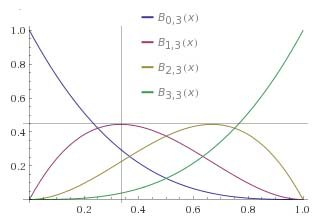
\includegraphics[width=95mm]{BP.jpg}
    \caption{Graph of Bernstein Polynomial of degree $3$}
    \label{fig:2}
\end{figure}
\newpage
We can see from figure \ref{fig:2}, a representation of a Bernstein basis with degree $3$. We can observe there is a symmetric relationship between the curves and this is occurred from $x$ and $(1-x)$ in the definition of the Bernstein basis. Each maximum of each $i$th curve occurs at $x=i/n$. (eg the maximum of $B_{1,3}$ occurs at $x=1/3$ as shown by the crosshairs in the graph) As $n$ increases and there are more curves to add up to $1$, they are going to drop down closer to the x-axis, resulting in somehow the contraction of each maximum point. What we mean by this, the `neighbourhood' of points around the maximum point will become wider. Plotting everything down, we can see a series of hills at which there is a decreasing gradient in $[1/3, 1/2]$ and then the gradient increases in $[1/2, 1]$.
\subsection{Overview of the proof}
For the above case to hold we need to show that $\lim_{n \rightarrow{\infty} }B_n(f)(x)=f(x)$ and that the convergence is uniform. As we have mentioned above, maximum point of each of the curves occurs at $x=\frac{i}{n}$, for $i=0,1,…,n$. This implies that the greatest contribution to the weighted average of points of each polynomial is split into partial sums where $\frac{i}{n}$ is closest to $x$. The main idea is that we need to show that our claim holds, because there exists some $\delta>0$ such that when we split the summation into two parts, one part will take all the points of
\begin{equation}
\left|\frac{i}{n}\ - x\right|< \delta    
\end{equation}
 and the second part all the points with 
 \begin{equation}
  \left|\frac{i}{n}\ - x\right|\geq \delta   
 \end{equation}
\subsubsection{Proof}
Firstly to understand the proof we need to be aware of some important equations which follow:
\begin{enumerate}
\item $i\binom{i}{n}=n\binom{n-1}{i-1}$ known as the absorption identity
\item $\sum_{i=0}^nB_{i,n}(x)=1$
\item $\sum_{i=0}^niB_{i,n}(x)=nx$
\item $\sum_{i=0}^ni(i-1)B_{i,n}(x)=n(n-1)x^2$
\end{enumerate}
We can prove $(3)$ as follows:
\begin{equation}
\sum_{i=0}^niB_{i,n}(x)=\sum_{i=0}^ni\binom{i}{n}x^i(1-x)^n-i=\sum_{i=1}^n\binom{n-1}{i-1}x^i(1-x)^{n-i}    
\end{equation}
as this follows from equation $(1)$. Also the summation starts from $1$ because the $0$th term is $0$.
\begin{equation}
n\left(\sum_{j=0}^{n-1}\binom{n-1}{j}x^{j+1}(1-x)^{(n-1)-j}\right)    
\end{equation}
we let $j=i-1$ and then the result follows by proper substitutions.
\begin{equation}
nx\left(\sum_{j=0}^{n-1}\binom{n-1}{j}x^{j+1}(1-x)^{(n-1)-j}\right)=nx\left(B_{j,n-1}(x)\right)=(nx)(1)=nx    
\end{equation}
and equation $(4)$ is proved similarly as $(3)$. So we begin the proof as follows:
\begin{align*}
&\sum_{i=0}^n(i-nx)^2B_{i,n}(x)\\
&=\sum_{i=0}^n(i(i-1)-(2nx-1)i+n^2 x^2)B_{i,n}(x)\\
&=n(n-1)x^2-(2nx-1)nx+n^2 x^2=nx(1-x)\leq\frac{1}{4n}\\   
\end{align*}
Using property $(4)$ and $(3)$ from the list above respectively we can see how the expression after the summation follows.
We know this statement is true, because $x(1-x)\leq\frac{1}{4}$ on $[0,1]$ since the maximum of this curve is at $\frac{1}{4}$. The next thing we do is that we divide by $n^2$, moving the $n^2$ inside the square brackets in the summation such as:
\begin{equation}
\sum_{i=0}^n\left(\frac{i}{n}-x\right)^2B_{i,n}(x)\leq\frac{1}{4n}    
\end{equation}
Now for any $x\in[0,1]$ we can choose $\delta_1>0$, and consider the sum of all $B_{i,n}(x)$ with $i$ such that $|\frac{i}{n}-x|\geq\delta_1$; that is, where $\frac{i}{n}$ is bounded away from $x$:
\begin{equation}
\sum_{i:|\frac{i}{n}-x|\geq\delta_1}(\frac{i}{n}-x)^2B_{i,n}(x)\leq\frac{1}{\delta^2}
\end{equation}
\begin{equation}
\sum_{i:|\frac{i}{n}-x|\geq\delta_1}(\frac{i}{n}-x)^2B_{i,n}(x)\leq(\frac{1}{\delta^2})(\frac{1}{4n})
\end{equation}
This inequality is true only for $i$ such that $|\frac{i}{n}-x|\geq\delta_1$. For those values $i$, $\frac{|\frac{i}{n}-x|}{\delta_1}\geq\ 1$ and therefore ,$\frac{|\frac{i}{n}-x|^2}{\delta_1^2}\geq\ 1$ justifying the introduction of $(\frac{i}{n}-x)^2$ and $\delta^2$ in the inequality. So if we fix $M\in[0,1]$ and we consider $|f(x)|<M$ on $[0,1]$, then:
\begin{equation}
\left|f(x)-\sum_{i:|\frac{i}{n}-x|\geq\delta_2}f(\frac{i}{n})B_{i,n}(x)\right|\leq\sum_{i:|\frac{i}{n}-x|\geq\delta_2}\left|f(x)-f(\frac{i}{n})\right|B_{i,n}(x)<\frac{2M}{4\delta^2n}=\frac{M}{2\delta^2n}
\end{equation}
Which holds only for $|\frac{i}{n}-x|\geq\delta_2$. For $i$ with $\frac{i}{n}$ closer to $x$, we can use uniform continuity of $f$ in the following way. Let $\epsilon>0$  and choose $\delta>0$ such that $|f(x)-f(\frac{i}{n})|<\frac{\epsilon}{2}$ when $|x- \frac{i}{n}|<\delta$ throughout $[0,1]$. So for $i$ with $|\frac{i}{n}-x|<\delta$:
\begin{equation}
\left|f(x)-\sum_{i:|\frac{i}{n}-x|<\delta}f(\frac{i}{n})B_{i,n}(x)\right|\leq\sum_{i:|\frac{i}{n}-x|<\delta}\left|f(x)-f(\frac{i}{n})\right|B_{i,n}(x)<\left(\frac{\epsilon}{2}\right)(1)= \frac{\epsilon}{2}   
\end{equation}
The theorem follows by combining the above two equations. So, let $\epsilon>0$ be given and choose $\delta$ so that the equation above holds, as discussed above. Then for that $\delta$, choose $n$ high enough so that $\frac{M}{(2\delta^2n)}<\epsilon/2$ and the left side of equation $(14)$ is less than $\frac{\epsilon}{2}$. It follows that for all $x\in[0,1]$:
\begin{equation}
\left|f(x)-\sum_{i=0}^nf(\frac{i}{n})B_{i,n}(x)\right|<\frac{\epsilon}{2}+\frac{\epsilon}{2}=\epsilon    
\end{equation}
\subsection{Properties of Bernstein Polynomials}
Bernstein basis polynomials have many useful properties, so we are going to show the most important ones.\paragraph{}
$(1)$\textbf{Recursive definition:}
We can consider a basis of degree n and can be defined as the sum of two Bernstein polynomials of degree $n-1$.
\begin{equation}
B_{i,n}(t)=(1-t)B_{i,n-1}(t)+tB_{i-1,n-1}(t)    
\end{equation}
Proof:
\begin{align*}
B_{i,n}(t)&=\binom{n}{i}t^i(1-t)^{n-1}=\left[\binom{n-1}{i}+\binom{n-1}{i-1}\right]t^i(1-t)^{n-i}\\
&=\binom{n-1}{i}t^i(1-t)^{n-i}+t\binom{n-1}{i-1}t^{i-1}(1-t)^{n-i}\\
&=(1-t)\binom{n-1}{i}t^i(1-t)^{n-1-i}+t\binom{n-1}{i-1}t^{i-1}(1-t)^{n-1-(i-1)}\\
&=(1-t)B_{i,n-1}(t)+tB_{i-1,n-1}(t)\\
\end{align*}
We can split the $\binom{n}{i}$ into $\binom{n-1}{i}+\binom{n-1}{i-1}$ using the Pascal’s identity. Then the result follows since $B_{i,n-1}(t)=\binom{n-1}{i}t^i(1-t)^{n-1-i}$ and $B_{i-1,n-1}(t)=t\binom{n-1}{i-1}t^{i-1}(1-t)^{n-1-(i-1)}$.\paragraph{}
$(2)$\textbf{Positivity:}
Bernstein basis polynomials are all considered positive if we take them in the interval $[0,1]$ and strictly positive on the interval $(0,1)$.\paragraph{}
Proof: This property is proved by induction based on the recursive property.
We can show with our base case that the polynomial is positive such that $B_{0,0}=1\geq0$ which holds. Then we will assume that for $b_{i,j}\geq0$ for all $i,j<n$ for some $n$. With the recursive property we have:
\begin{equation}
B_{i,n}(t)=(1-t)B_{i,n-1}(t)+tB_{i-1,n-1}(t)    
\end{equation}
Hence $b_{i,n}(t)\geq0$ in the closed interval since the right hand side is composed from positive numbers. So we can confirm this to all Bernstein polynomials on the closed interval. The same result follows on the open interval as well.\paragraph{}
\textbf{$(3)$Bernstein polynomials form a partition of unity:}
Consider a set of funtions $f_i(t)$. this is said to be a partition of unity if and only if their sum is equal to $1$ for all values of $t$. So, the $k + 1$ Bernstein basis polynomials for a Bernstein polynomial of degree $k$ form a partition of unity. That is:
\begin{equation}
B_k(t)=\sum_{i=0}^nB_{i,n}(t)= B_{0,n}(t)+B_{1,n}(t)+...+B_{n,n}(t)=1,  0\leq t\leq 1  
\end{equation}\paragraph{}
Proof:The following property is used to explain this proof at which we are going to proof as well.
\begin{equation}
B_n(t)=B_{n-1}(t)    
\end{equation}
This is again proved using the recursive property:
\begin{align*}
B_n(t)&=\sum_{i=0}^n((1-t)B_{i,n-1}(t)+tB_{i-1,n-1}(t))\\
&=(1-t)\left[\sum_{i=0}^nB_{i,n-1}+B_{n,n-1}\right]+t\left[\sum_{i=0}^nB_{i-1,n-1}(t)+B_{-1,n-1}(t)\right]\\
&=(1-t)\sum_{i=0}^{n-1}B_{i,n-1}(t)+t\sum_{i=0}^{n}B_{i-1,n-1}(t)\\
&=(1-t)\sum_{i=0}^{n-1}B_{i,n-1}(t)+t\sum_{i=0}^{n-1}B_{i,n-1}(t)\\
&=\sum_{i=0}^{n-1}B_{i,n-1}(t)\\
&=B_{n-1}(t)
\end{align*}\paragraph{}
Again using the above property bwe can use induction. So, our base case $B_0(t)=\sum_{i=0}^nB_{i,n}(t)=B_{0,0}(t)=1$ and this follows for all the polynomials since $1=B_0(t)=B_1(t)=B_2(t)=..=B_n(t)$. Hence, $B_n(t)=1$ for all $n\geq0$ in $[0,1]$.
\section{B\'ezier Curves}\label{sec:bec}
A \emph{B\'ezier Curve} is a parametric curve that uses the Bernstein Polynomial as a basis; % (http://web.mit.edu/hyperbook/Patrikalakis-Maekawa-Cho/ode12.html).
i.e.\ for a set of vectors $\mathbf{r}_0, \mathbf{r}_1, \dots, \mathbf{r}_n$ we have the B\'ezier curve
\begin{equation} \label{eq:bec:1}
\mathbf{r}(t) = \sum_{i=0}^{n} B_{i,n}(t) \mathbf{b}_i
\end{equation}
where $B_{i,n}(t)$ is the \emph{Bernstein Polynomial} defined on $\left[0,1 \right]$ as follows.
\[
  B_{i,n}(t) = \binom{n}{i} t^i (1 - t)^{n-i}
\]

We recall that as, $B_{i,n}(t)$ is a binomial coefficient.
Then we have that  $\sum_{i=0}^n B_{i,n}(t)$ = 1.
Thus we can percieve the B\'ezier curve as defined in (\ref{eq:bec:1}) as a weighted mean over the points $\mathbf{b}_0, \mathbf{b}_1, \dots, \mathbf{b}_n$, with $B_{i,n}$ being the weight on point $\mathbf{b}_i$. %(see figure of graph of bernstein polynomials).
It follows that every point on the B\'ezier curve lies in the convex hull of the points $\mathbf{b}_0, \mathbf{b}_1, \dots, \mathbf{b}_n$; i.e.\ the smallest convex figure containing the points.

Now we will consider some examples of B\'ezier curves to understand their behaviour.
The simplest B\'ezier curve that we can talk about is the linear curve between two points $\mathbf{b}_0$ and $\mathbf{b}_1$.
The parametric equation for this is given as follows.
\begin{equation}
  \label{eq:bec:2}
  \mathbf{r}(t) = \mathbf{b}_0 (1 - t) + \mathbf{b}_1 t
\end{equation}
We notice that the curve defined in (\ref{eq:bec:2}) is a line between $\mathbf{b}_0$ and $\mathbf{b}_1$ with $\mathbf{r}(0) = \mathbf{b}_0$ and $\mathbf{r}(1) = \mathbf{b}_1$. This curve is depicted in Figure \ref{fig:bec:1}.


\begin{figure}
  \centering
  \begin{tikzpicture}
    \filldraw
    (0,0) circle (1pt) node [left] {$\mathbf{b}_0$} --
    (1.5,1) circle (1pt) node [below] {$\mathbf{r}(\frac{1}{2})$} --
    (3,2) circle (1pt) node [right] {$\mathbf{b}_1$};
  \end{tikzpicture}
  \caption{A linear B\'ezier curve}
  \label{fig:bec:1}
\end{figure}
  
Notice that when $t = \frac{1}{2}$ the position vector $\mathbf{r}$ is the midpoint of the endpoints.
This agrees with our notion of $\mathbf{r}$ as the weighted mean of the endpoints.

In a similar manner, we can talk about B\'ezier curves that are quadratic (controlled by three points) and cubic (controlled by four points). We have the parametric equation of the cubic B\'ezier curve below.

\begin{equation}
  \label{eq:bec:3}
  \mathbf{r}(t) = (1-t)^3 \mathbf{b}_0 + t(1-t)^2 \mathbf{b}_1 + t^2(1-t) \mathbf{b}_2 + t^3 \mathbf{b}_3
\end{equation}

The corresponding curve is depicted in Figure \ref{fig:bec:2}.

\begin{figure}
  \centering
  \begin{tikzpicture}
    \coordinate (A) at (0,0);
    \coordinate (B) at (2,3);
    \coordinate (C) at (5,3);
    \coordinate (D) at (4,0);
    \draw (A) .. controls (B) and (C) .. (D);
    \filldraw [dotted]
    (A) circle (1pt) node [left] {$\mathbf{b}_0$} --
    (B) circle (1pt) node [left] {$\mathbf{b}_1$};
    \filldraw [dotted]
    (C) circle (1pt) node [right] {$\mathbf{b}_2$} --
    (D) circle (1pt) node [right] {$\mathbf{b}_3$};
  \end{tikzpicture}
  \caption{A cubic B\'ezier curve}
  \label{fig:bec:2}
\end{figure}

A simple computation shows us that $\mathbf{r} ' (0) = \lambda(\mathbf{b}_1 - \mathbf{b}_0)$ for some $\lambda \in \mathbb{R}$; by the properties of the product rule, this will hold a B\'ezier curve of any order.
Similarly if a B\'ezier curve has order $n$, we notice that $\mathbf{r} ' (1) = \mu (\mathbf{b}_n - \mathbf{b}_{n-1})$ for some $\mu \in \mathbb{R}$.
This shows that $\mathbf{r}$ leaves $\mathbf{b}_0$ moving towards $\mathbf{b}_1$ and arrives at $\mathbf{b}_n$ from the direction of $\mathbf{b}_{n-1}$.
The aforementioned is visually depicted in Figure \ref{fig:bec:2}.

\subsection{Recursive Property of B\'ezier Curves.}
\label{sec:bec:1}

B\'ezier curves are particularly useful because of they are \emph{recursive}, a property that is attributed to Paul de Casteljau \cite{casselman08}.
It will not be proved here.

Consider Figure \ref{fig:bec:3}.
We find the three midpoints between adjacent control points and label them accordingly.
We do this again to find the pair of midpoints between the aforementioned midpoints and finally find the midpoint $\mathbf{c}$ between this pair.
Studying the figure will make this clear.

Immediately we notice that $\mathbf{c}$ seems to be on the curve.
This is indeed the case.
In fact, the property described at the beginning of this subsection asserts that the segment of the curve between $\mathbf{b}_0$ and $\mathbf{c}$ is itself an independent B\'ezier curve.
This B\'ezier curve has control points $\mathbf{h}_{01}$ and $\mathbf{h}_{012}$, as may be guessed by studying the figure.
Similarly, the segment between $\mathbf{c}$ and $\mathbf{b}_3$ is a B\'ezier curve with control points $\mathbf{h}_{123}$ and $\mathbf{h}_{23}$.

de Casteljau's algorithm uses this property to draw B\'ezier curves by recursively breaking down each B\'ezier curve into two segments in the way that we have described above.
This makes B\'ezier curves very easy to render by computers.
Rendering is done by applying de Casteljau's algorithm recursively breaking each curve into two curves till the control points of the curve are approximately collinear, then we draw a line through the points.
This is particularly suited to binary machines that are prevalent today as it is facilitated by division by two.

One particular use of B\'ezier curves is in designing fonts. The designer need just select control points and is able to generate a smooth curve.
TrueType fonts use quadratic B\'ezier curves.
Rendering quadratic B\'ezier curves is done by an algorithm similar to that of cubic curves.
Other fonts such as PostScript and some OpenType fonts use quadratic B\'ezier curves.
% cite wikipedia

In computer graphics, we tend to use only quadratic and cubic B\'ezier curves as higher order curves are computationally expensive.
If we want a curve that is modelled by a higher order, quadratic or cubic curves are often stitched together in sequence to produce the effect.

\begin{figure}
  \centering
  \begin{tikzpicture}
    \coordinate (A) at (0,0);
    \coordinate (B) at (3,9);
    \coordinate (C) at (6,8);
    \coordinate (D) at (12,2);
    \coordinate (h01) at ($0.5*(A) + 0.5*(B)$);
    \coordinate (h12) at ($0.5*(B) + 0.5*(C)$);
    \coordinate (h23) at ($0.5*(C) + 0.5*(D)$);
    \coordinate (h012) at ($0.5*(h01) + 0.5*(h12)$);
    \coordinate (h123) at ($0.5*(h12) + 0.5*(h23)$);
    \coordinate (c) at ($0.5*(h012) + 0.5*(h123)$);
    \draw (A) .. controls (B) and (C) .. (D);
    \draw [gray]
    (A) circle (1pt) node [left] {$\mathbf{b}_0$} --
    (h01) circle (1pt) node [left] {$\mathbf{h}_{01}$} --
    (B) circle (1pt) node [left] {$\mathbf{b}_1$} --
    (h12) circle (1pt) node [above] {$\mathbf{h}_{12}$} --
    (C) circle (1pt) node [right] {$\mathbf{b}_2$} --
    (h23) circle (1pt) node [right] {$\mathbf{h}_{23}$} --
    (D) circle (1pt) node [right] {$\mathbf{b}_3$};
    \filldraw[dotted]
    (h01) circle (1pt) --
    (h012) circle (1pt) node [left] {$\mathbf{h}_{012}$} --
    (h12) circle (1pt);
    \filldraw[dotted]
    (h12) circle (1pt) --
    (h123) circle (1pt) node [right] {$\mathbf{h}_{123}$} --
    (h23) circle (1pt);
    \filldraw[dotted]
    (h012) circle (1pt) --
    (c) circle (1pt) node [above] {$\mathbf{c}$} --
    (h123) circle (1pt);
  \end{tikzpicture}
  \caption{Constructing a cubic B\'ezier curve}
  \label{fig:bec:3}
\end{figure}

\section{Weierstrass Approximation Theorem}\label{sec:wet}
The Weierstrass approximation theorem states that:
\newline
 If $F(x)$ is any continuous function in the interval $[0,1]$, it is always possible, regardless how small $\epsilon$, to determine a polynomial $E_n=a_0x^n+a_1x^{n-1}+\dots+a_n$ of degree $n$ high enough such that we have 
\begin{equation*}
    |F(x)-E_n(x)|<\epsilon
\end{equation*}
for every point in the interval under consideration.\cite{bertrand15}
\subsection{Proof using Bernstein Polynomial}\label{subsec:pfd}
The curve $f(x)=e^{-\frac{1}{x^2}}$ is one of the cases when a function has a Taylor series expansion at some point and the convergence of the series may be extremely slow to compute. However, there are various ways on how we approximate a function in a fixed point. Ideally, we would like a method that could compute a uniform approximation of a continuous function by a polynomial of some degree. This is not the case, so instead we can take a finite set of points on closed interval and take this uniform approximation to our function as we increase the number of points in the interval so that the polynomials are uniformly dense in the set of continuous polynomials $C( [a,b] , \mathbb{R})$ with respect to the sup-norm. The Weierstrass Approximation Theorem tells us that this could be done with every continuous function, but it does not tell us how to get the actual polynomial approximation. We’ll see that a sequence of Bernstein polynomials is the actual polynomials that uniformly converge to our function.\paragraph{}
Consider $f \in C([a,b] ,\mathbb{R})$. Then there is a sequence of polynomials $p_n(x)$ that converges uniformly to $f(x)$ on $[a, b]$.\paragraph{}
We want to show that for any function in $C( [a,b] ,\mathbb{R})$ there exists a sequence of polynomials $p_n$ such that $p_n$ converges to $f$ uniformly. To show this, we will actually define a map $\phi$ that maps functions from $[a,b]$ to $[0,1]$. So define, $\phi:C([a,b])\rightarrow{}C([0,1])$ by $(\phi f)(t)=f(a+(b-a)t)$. We know that $\phi$ by its definition that is linear and invertible and has inverse:
\begin{equation}
(\phi^{-1}f)(t)=f\left(\frac{a-t}{b-a}\right)    
\end{equation}
If $p$ is dense enough in $C([0,1])$ and when we refer to ‘dense’ we mean if it is contracted well enough in the interval , then for any $f\in C([a,b])$  , we have $p_n \rightarrow{} \phi f\in C([0,1])$ . Hence $\phi^(-1)p_n$ converges to $f$ in $C([a,b])$ . To show $p_n$ is dense in $C([ 0,1])$ , we will use Bernstein’s polynomials. Recall that a Bernstein basis of polynomials forms a partition of unity such that:
\newline
$B_n(t)=\sum_{i=0}^nB_{i,n}(t)=B_{0,n}(t)+B_{1,n}(t)+...+B_{n,n}(t)=1, 0\leq t\leq1$\newline 
So we can find the difference between f and the nth polynomial as:
\begin{align*}
&B_n(t;f)-f(t)=\sum_{i=0}^nf\left(\frac{i}{n}\right)B_{i,n}(t)-\sum_{i=0}^nf(t)B_{i,n}(t)\\
&=\sum_{i=0}^n\left[f\left(\frac{i}{n}\right)-f(t)\right]B_{i,n}(t)\\
\end{align*}
Now we have to consider the supremum with respect to the absolute value of the equation to get:
\begin{equation}
||B_n(\cdot;f)-f(t)||=\sup_{0\leq t\leq 1}\left[\sum_{i=0}^n\left|f\left(\frac{i}{n}\right)-f(t)\right|B_{i,n}(t)\right]    
\end{equation}
Where $B_n(t;f)$ denotes the polynomial at $t$ and $B_n(\cdot;f)$ denotes the polynomial at the whole interval $[0,1]$. We know f is uniformly continuous, hence 
\begin{equation}
(\forall\epsilon>0)(\exists\delta>0)(|x-y|<\delta\implies|f(x)-f(y)|<\epsilon), \forall x,y\in[0,1]    
\end{equation}
To find the supremum we need to split the terms as follow:
\begin{align*}
&I(t)=\left\{k|0\leq k\leq n and \left|t-\left(\frac{k}{n}\right)\right|<\delta\right\}\\
&J(t)=\left\{k|0\leq k\leq n and \left|t-\left(\frac{k}{n}\right)\right|\geq\delta\right\}\\
\end{align*}
And then combining all these we have:
\begin{align*}
&||B_n(\cdot;f)-f(t)||\leq\epsilon\sup_{0\leq t\leq 1}\left[\sum_{k\in I(t)}B_{k,n}(t)\right]+\sup_{0\leq t\leq 1}\left[\sum_{k\in J(t)}\left|\left(\frac{k}{n}\right)-f(t)\right|B_{k,n}(t)\right]\\
&\leq\epsilon+2||f||\sup_{0\leq t\leq 1}\left[\sum_{k\in J(t)}B_{k,n}(t)\right]\\
\end{align*}
Because we have that $\epsilon$ times the summation of $B_{k,n}(t)$ is equal to $\epsilon$ since the summation of the polynomial is equal to $1$.
So $\epsilon$ times $1$ is equal to $\epsilon$.
Now, $\left[ t-\left( \frac{k}{n} \right) \right]^2 \geq \delta^2$ for $k\in J(x)$ we can estimate the right-hand side of the above inequality as follows:
\begin{align*}
&\sup_{0\leq t\leq 1}\left[\sum_{k\in J(t)}B_{k,n}(t)\right]\leq\frac{1}{\delta^2}\sup_{0\leq t\leq 1}\left[\sum_{k\in J(t)}\left(t-\frac{k}{n}\right)^2 B_{k,n}(t)\right]\\
&\leq\frac{1}{\delta^2}\sup_{0\leq t\leq 1}\left[\sum_{k=0}^n\left(t^2-\frac{2kt}{n}+\frac{k^2}{n^2}\right)^2 B_{k,n}(t)\right]\\
&\leq\frac{1}{\delta^2}\sup_{0\leq t\leq 1}\left[t^2-B_n(t;1)-2tB_n(t;t)+B_n(t;t^2)\right]\\
\end{align*}
Where the summation over $\delta^2\leq1$. To evaluate these above Bernstein polynomials $B_n(t;1)$, $B_n(t;t)$ and $B_n(t;t^2)$ we’ll differentiate twice with respect to $t$ and take the first and second derivative of the binomial expansion of the polynomials.
\begin{align*}
&\sum_{k=0}^n\binom{n}{k}t^ky^{n-k}=(t+y)^n\\
&\sum_{k=0}^n\frac{k}{n}\binom{n}{k}t^ky^{n-k}=t(t+y)^{n-1}\\
&\sum_{k=0}^n\left(\frac{k}{n}\right)^2\binom{n}{k}t^ky^{n-k}=\left(\frac{n-1}{n}\right)t^2(t+y)^n-2\frac{t}{n}(t+y)^{n-1}\\
\end{align*}
If we let $y=1-t$ (to satisfy the definition of a Bernstein polynomial) gives:
\begin{align*}
&B_n(t;1)=1\\
&B_n(t;t)=t\\
&B_n(t;t^2)=\left(\frac{n-1}{n}\right)t^2+\left(\frac{1}{n}\right)t\\
\end{align*}
for $n\geq1$. Plugging these back in to our inequality gives:
\begin{equation}
||B_n(\cdot;f)-f(t)||\leq\epsilon+\frac{||f||}{2n\delta^2}    
\end{equation}
And then we take the limit superior to get
\begin{equation}
\limsup_{n\rightarrow{\infty}}||B_n(\cdot;f)-f(t)||\leq\epsilon    
\end{equation}
Since $\epsilon$ is arbitrary, it follows $\limsup_{n\rightarrow{\infty}}||B_n(\cdot;f)-f(t)|| = 0$, so $p_n = B_n(\cdot;f)$ converge uniformly to $f$.


\subsection{Proof by Bernstein using Probability Theory}\label{subsec:pbb}
Here, we will be looking at Bernstein's take on proving the Weierstrass Approximation theorem and it turned out to be the simplest proof yet.
To start with the proof, we will consider an event $A$, whose probability of it happening is equal to $x$. 
Then, we assume $n$ experiments are conducted and the player is to be paid the sum $F(\frac{m}{n})$, if the event occurs $m$ times, where $F$ is a continuous function.\cite{bertrand15}
Under these circumstances, we will now calculate the expected value of the sum paid to the player, which is:
\begin{equation*}
    E_n = \sum_{m=0}^{n}F\left(\frac{m}{n}\right)\cdot{m\choose n}\cdot x^n\cdot(1-x)^{n-m}
\end{equation*}
Due to continuity of $F$, we can have some number, $\delta>0$, such that we have the following inequality,
\begin{equation*}
|x-x_0|\leq\delta
\end{equation*}
So by definition of continuity, for all $\epsilon>0$, we have
\begin{equation*}
    |F(x)-F(x_0)|<\frac{\epsilon}{2};
\end{equation*}
Considering the interval for $(x-\delta,x+\delta)$, and if $\overline{F}(x)$ is the maximum and $\underline{F}(x)$ is the minimum of $F(x)$ in the interval, then we have
\begin{equation}\label{eqn:eps}
    \overline{F}(x)-F(x)<\frac{\epsilon}{2}, F(x)-\underline{F}(x)<\frac{\epsilon}{2}
\end{equation}
Then, let $\eta$ be the probability that the inequality is $|x-\frac{m}{n}|>\delta$.
Also, we will set the maximum of $|F(x)|$ in the interval $[0,1]$ be $L$.
Looking back at the function $E_n(x)$,
\begin{align*}
    E_n(x) &= \mathbb{E}\left(F\left(\frac{m}{n}\right)\cdot1\right) \\
    &= \mathbb{E}\left(F\left(\frac{m}{n}\right)\cdot \mathbb{I}\left[|x-\frac{m}{n}|>\delta\right]\right) + \mathbb{E}\left(F\left(\frac{m}{n}\right)\cdot \mathbb{I}\left[|x-\frac{m}{n}|<\delta\right]\right),\\
\end{align*}
Since we have the following inequality,
\begin{align*}
    -L\cdot\eta&<\mathbb{E}\left(F\left(\frac{m}{n}\right)\cdot \mathbb{I}\left[|x-\frac{m}{n}|>\delta\right]\right)<L\cdot\eta\\
    \underline{F}(x)\cdot(1-\eta)&<\mathbb{E}\left(F\left(\frac{m}{n}\right)\cdot \mathbb{I}\left[|x-\frac{m}{n}|<\delta\right]\right)<\overline{F}(x)\cdot (1-\eta)
\end{align*}
We then have,
\begin{equation*}
 \underline{F}(x)\cdot(1-\eta)-L\cdot\eta<E_n(x)<\overline{F}(x)\cdot (1-\eta)+L\cdot\eta 
\end{equation*}
 By the Law of Large Numbers from probability theory, we have that $\eta$ tends to zero as $n$ gets significantly large.
Therefore, we can take $n$ large enough such that 
\begin{equation*}
\eta<\frac{\epsilon}{4L}
\end{equation*}
Then, we get the following inequality
\begin{equation*}
    F(x)+(\underline{F}(x)-F(x))-\eta(L+\underline{F}(x))<E_n(x)< F(x)+(\overline{F}(x)-F(x))+\eta(L-\overline{F}(x))
\end{equation*}
and so using the inequality (\ref{eqn:eps}),
\begin{equation*}
    F(x)-\frac{\epsilon}{2}-\frac{2L}{4L}\epsilon<E_n(x)<F(x)+\frac{\epsilon}{2}+\frac{2L}{4L}\epsilon
\end{equation*}
Hence, we get
\begin{equation*}
    |F(x)-E_n(x)|<\epsilon
\end{equation*}
Since we know $E_n$ is clearly a polynomial with degree $n$, so the theorem is proved.


\newpage
\nocite{casselman08}
\nocite{tuladhar_2016}
\nocite{gt2014}
\nocite{rvk}
\nocite{bertrand15}
\nocite{farouki2012bernstein}
\nocite{pinkus2000weierstrass}
\nocite{o'connor_robertson_2010}
\bibliographystyle{ieeetr}
\bibliography{references}
\end{document}
%%% Local Variables:
%%% mode: latex
%%% TeX-master: t
%%% End: